%%%%%%%%%%%%%%%%%%%%%%%%%%%%%%%%%%%%%%%%%%%%%%%%
%%   TEMPLATE MAIN FILE                       %%
%%%%%%%%%%%%%%%%%%%%%%%%%%%%%%%%%%%%%%%%%%%%%%%%

\documentclass[10pt,reqno,sumlimits]{amsart}
\usepackage{amssymb}
\usepackage{epsfig}
\usepackage{multirow}
\usepackage{graphics}
\usepackage{graphicx}
\usepackage{subfigure}
\usepackage{url}
%\textwidth 6.2in
%\oddsidemargin.20in
%\evensidemargin.35in
%%\lineskip 1in
%%\baselineskip.55cm

% Read in specially defined commands
% Change margins and baselinestretch in draft mode
\def\draft{
% make margins smaller
\addtolength{\oddsidemargin}{-0.5in}
\addtolength{\topmargin}{-0.65in}
\addtolength{\textheight}{1in}
\addtolength{\textwidth}{1.5in}
% A more reasonable baselinestretch, is still nearly doublespaced.
\def\baselinestretch{1.4}
}

%\vfuzz2pt % Don't report over-full v-boxes if over-edge is small
%\hfuzz2pt % Don't report over-full h-boxes if over-edge is small

%%%%%%%%%%%%%%%%%%%%%%%%%%%%%%%%%%%%%%%%%%%%%%%%%%%%%%%%
%%              Theorems                               %
%%%%%%%%%%%%%%%%%%%%%%%%%%%%%%%%%%%%%%%%%%%%%%%%%%%%%%%%
\theoremstyle{plain}
\newtheorem{theorem}{Theorem}
\newtheorem{corollary}[theorem]{Corollary}
\newtheorem{lemma}[theorem]{Lemma}
\newtheorem{proposition}[theorem]{Proposition}
\newtheorem{conjecture}[theorem]{Conjecture}

\theoremstyle{definition}
\newtheorem{remark}[theorem]{Remark}
\newtheorem{definition}[theorem]{Definition}
\newtheorem{example}[theorem]{Example}
\newtheorem{notation}{Notation}

%%%%%%%%%%%%%%%%%%%%%%%%%%%%%%%%%%%%%%%%%%%%%%%%%%%%%%%%
%%      Definitions and Commands                       %
%%%%%%%%%%%%%%%%%%%%%%%%%%%%%%%%%%%%%%%%%%%%%%%%%%%%%%%%
\newcommand{\A}{{\mathbb A}}
\newcommand{\R}{{\mathbb R}}
\newcommand{\Q}{{\mathbb Q}}
\newcommand{\C}{{\mathbb C}}
\newcommand{\D}{{\mathbb D}}
\newcommand{\Z}{{\mathbb Z}}
\newcommand{\h}{{\mathbb H}}
\newcommand{\CP}{{\mathbb C}{\mathbb P}}
\newcommand{\I}{{\mathbb I}}
\newcommand{\N}{{\mathbb N}}
%
\newcommand{\calA}{{\mathcal A}}
\newcommand{\calB}{{\mathcal B}}
\newcommand{\calC}{{\mathcal C}}
\newcommand{\calD}{{\mathcal D}}
\newcommand{\calE}{{\mathcal E}}
\newcommand{\calF}{{\mathcal F}}
\newcommand{\calG}{{\mathcal G}}
\newcommand{\calH}{{\mathcal H}}
\newcommand{\calI}{{\mathcal I}}
\newcommand{\calK}{{\mathcal K}}
\newcommand{\calM}{{\mathcal M}}
\newcommand{\calO}{{\mathcal O}}
\newcommand{\calP}{{\mathcal P}}
\newcommand{\calR}{{\mathcal R}}
\newcommand{\calS}{{\mathcal S}}
\newcommand{\calL}{{\mathcal L}}
\newcommand{\calX}{{\mathcal X}}
\newcommand{\calU}{{\mathcal U}}
\newcommand{\calV}{{\mathcal V}}
\newcommand{\calZ}{{\mathcal Z}}
%
\newcommand{\ggoth}{{\mathfrak  g}}
\newcommand{\ugoth}{{\mathfrak  u}}
\newcommand{\hgoth}{{\mathfrak  h}}
%%
\newcommand{\1}{{\bf 1}}
\newcommand{\acts}{{\circlearrowright}}
\newcommand{\ex}[1]{{e^{#1}}}
\newcommand{\dd}[2]{\frac{\partial #1}{\partial #2}}
\newcommand{\iso}{\stackrel{\simeq}{\longrightarrow}}
\newcommand{\spinc}{$\text{spin}^c$}
\newcommand{\Dirac}{\not\!\!D}
\newcommand{\inc}{\hookrightarrow}
%%
\newcommand{\Aut}{\operatorname{Aut}}
\newcommand{\Hom}{\operatorname{Hom}}
\newcommand{\Hor}{\operatorname{Hor}}
\newcommand{\Ext}{\operatorname{Ext}}
\newcommand{\End}{\operatorname{End}}
\newcommand{\Map}{\operatorname{Map}}
\newcommand{\Diff}{\operatorname{Diff}}
\newcommand{\Tr}{\operatorname{Tr}}
\newcommand{\Lie}{\operatorname{Lie}}
\newcommand{\ad}{{\operatorname{ad\,}}}
\newcommand{\sign}{{\operatorname{sign}}}
\newcommand{\grad}{{\operatorname{grad}}}
\newcommand{\coker}{{\operatorname{coker}}}
\newcommand{\dett}{{\operatorname{det}}}
\newcommand{\ch}{{\operatorname{ch}}}
\newcommand{\rk}{{\operatorname{rk}}}
\newcommand{\maxx}{{\operatorname{max}}}
\newcommand{\minn}{{\operatorname{min}}}
\newcommand{\id}{{\operatorname{id}}}
\newcommand{\ind}{{\operatorname{ind}}}
\newcommand{\Ind}{{\operatorname{Ind}}}
\newcommand{\spann}{{\operatorname{span}}}
\newcommand{\Spin}{{\operatorname{Spin}}}
\newcommand{\Pin}{{\operatorname{Pin}}}
\newcommand{\im}{{\operatorname{Im}}}
\renewcommand{\Im}{{\operatorname{Im}}}
\newcommand{\dimm}{{\operatorname{dim}}}
\newcommand{\cl}{{\operatorname{cl}}}
%%
\newcommand{\tM}{{\tilde{M}}}
\newcommand{\tC}{{\tilde{C}}}
\newcommand{\tE}{{\tilde{E}}}
\newcommand{\tF}{{\tilde{F}}}
\newcommand{\talpha}{{\tilde{\alpha}}}
%%
\newcommand{\zbar}{\overline{z}}
\newcommand{\wbar}{\overline{w}}
\newcommand{\phibar}{\overline{\phi}}
\newcommand{\psibar}{\overline{\psi}}
\newcommand{\Bbar}{\overline{B}}
\newcommand{\Cbar}{\overline{C}}
\newcommand{\inv}{^{-1}}
%%      
\newcommand{\rb}[1]{\raisebox{0pt}[0pt][0pt]{#1}}
\newsavebox{\savepar}
\newenvironment{boxit}{\begin{lrbox}{\savepar}\begin{minipage}[b]{.5in}}
{\end{minipage}\end{lrbox}\fbox{\usebox{\savepar}}}
%%\newcommand{\ip}[1]{\langle\! #1 \! \rangle}
\newcommand{\ip}[1]{\langle #1 \rangle}
\newcommand{\norm}[1]{\| #1 \|}
%
%\newcommand{\remark}{{\tt ?}\marginpar{\Large\centering ?}}
\newcommand{\rremark}{\marginpar{\Large\centering ?}}
\newcommand{\Remark}[1]{\textsc{\tiny{[#1]}}\rremark}
\newcommand{\todo}{\textsc{Todo!}\marginpar{\Large\centering !}}
%
\numberwithin{equation}{section}
\renewcommand{\theequation}{{\thesection{.}}\arabic{equation}}
\newcounter{dummy}
%
%%%%%%%%%%%%%%%%%%%%%%%%%%%%%%%%%%%%%%%%%%%%%%%%%%%%%%%
\begin{document}

\title[Midterm]{Discrete Math II}
\author{Joe Smith}


%\begin{abstract}
%The abstract
%\end{abstract}

\maketitle

%\tableofcontents

%%%%%%%%%%%%%%%%%%%%%%%%%%%%%%%%%%%%%%%%%%%%%%%%%%%%%%%

\section {}
Construct a relation on the set ${a, b, c, d}$ that is\\
%a
\begin{figure}[htbp]
\centerline{
    \mbox{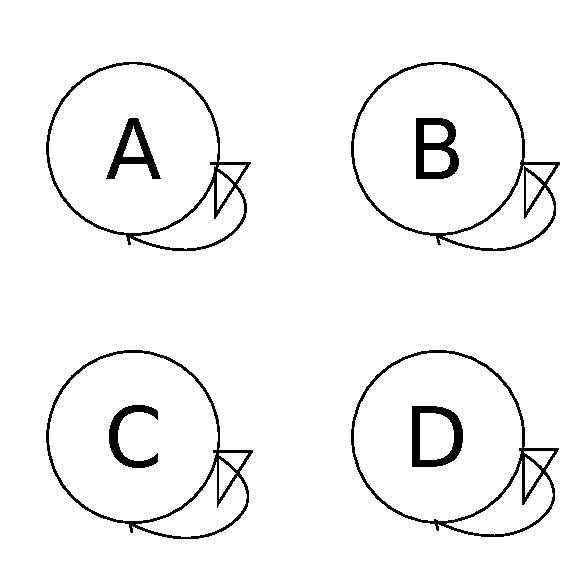
\includegraphics[width=1.5in]{1_a.pdf}}
  }
  \caption{reflexive, symmetric, but not transitive}
\end{figure}

%b
\begin{figure}[htbp]
\centerline{
    \mbox{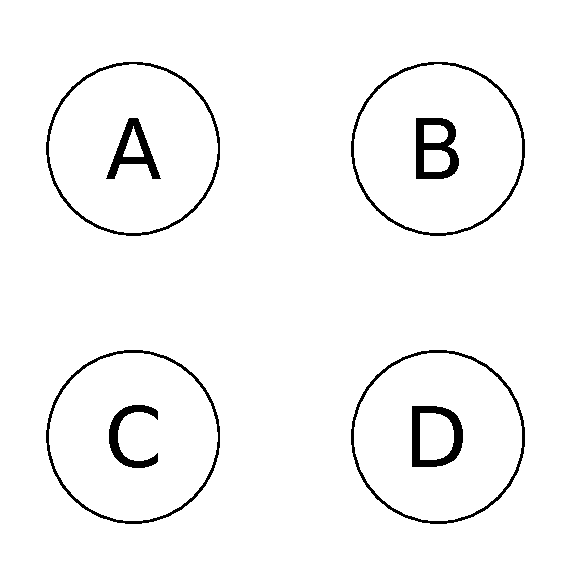
\includegraphics[width=1.5in]{1_b.pdf}}
  }
  \caption{irreflexive, symmetric, and transitive}
\end{figure}

%c
\begin{figure}[htbp]
\centerline{
    \mbox{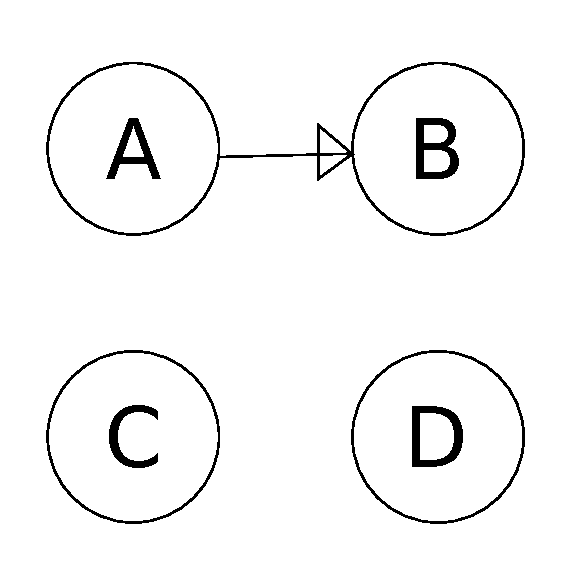
\includegraphics[width=1.5in]{1_c.pdf}}
  }
  \caption{irreflexive, antisymetric, and not transitive}
\end{figure}

%d
\begin{figure}[htbp]
\centerline{
    \mbox{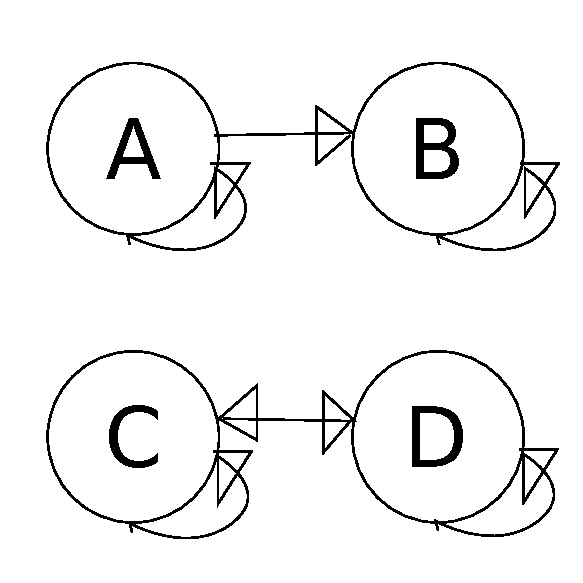
\includegraphics[width=1.5in]{1_d.pdf}}
  }
  \caption{reflexive, neither symmetric nor antisymetric, and transitive}
\end{figure}

%e
\begin{figure}[htbp]
\centerline{
    \mbox{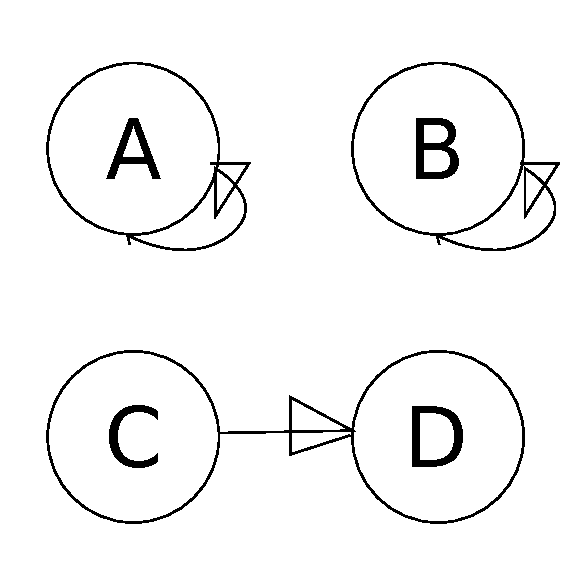
\includegraphics[width=1.5in]{1_e.pdf}}
  }
  \caption{neither reflexive, irreflexive, symmetric, antisymmetric, nor transitive}
\end{figure}
\clearpage

\section{}
\subsection{}
\begin{figure}[h]
\centerline{
    \mbox{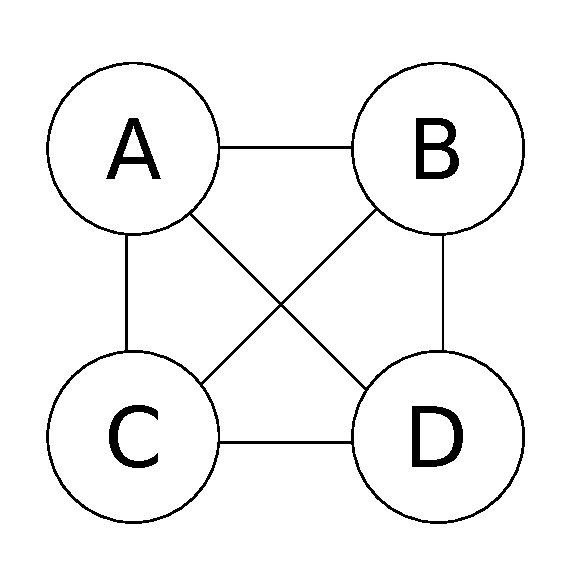
\includegraphics[width=1.5in]{2_a.pdf}}
  }
  \caption{Complete Graph $K_4$}
\end{figure}
\subsection{}
\[ \left( \begin{array}{ccccc}
\  & a & b & c & d \\
a & 0 & 1 & 1 & 1 \\
b & 1 & 0 & 1 & 1 \\
c & 1 & 1 & 0 & 1 \\
d & 1 & 1 & 1 & 0\end{array} \right) \]
\subsection{}
$A^3 =$
\[ \left( \begin{array}{ccccc}
\  & a & b & c & d \\
a & 6 & 7 & 7 & 7 \\
b & 7 & 6 & 7 & 7 \\
c & 7 & 7 & 6 & 7 \\
d & 7 & 7 & 7 & 6\end{array} \right) \]
\subsection{}
All paths of length 3 between vertices $a$ and $b$: $abab$, $abcb$, $abdb$, $acab$, $acdb$, $adab$, $adcb$\\


%3
\section{}
Which of these collections of subsets are partitions of $\mathbb{Z}$\\
\subsection{}
The even and odd integers, when taken as a union, return the whole set of intergers, and thus form a partition.
\subsection{}
The union of the sets of positive and negative integers are not a partition of $\mathbb{Z}$, since that does not include $0$.
\subsection{}
This forms a partion, as every integer will either be divisible by three, or have a remainder of one or two.
\subsection{}
This is a partition, as the absolute value of all numbers not exceeding 100 is $(-100, 100)$, and the set also includes all numbers less than $-100$ and greater than $100$.
\subsection{}
This is a partition, as every number that is divisible by three but not an even number will have a remainder of three when divided by six.

%4
\section{}


%5
\section{}
\subsection{}
To show a relation is poset, it must be reflexive, antisymmetric, and transitive.

$(\mathbb{N}, |)$ is reflexive: $\forall a \in \mathbb{N}, ak = a$ where $k = 1$\\
Antisymmetric: If one has $ak = b$, and $bk = a$, then $a = b/k$ and $b = a/k$. THe only way $bk=b/k$ is if $k = 1$, which means $a = b/1$, thus $a = b$.\\
Transitive: If $ak=b$ and $bj= c$ then $(ak)j = c$.

\subsection{}
\begin{figure}[htbp]
\centerline{
    \mbox{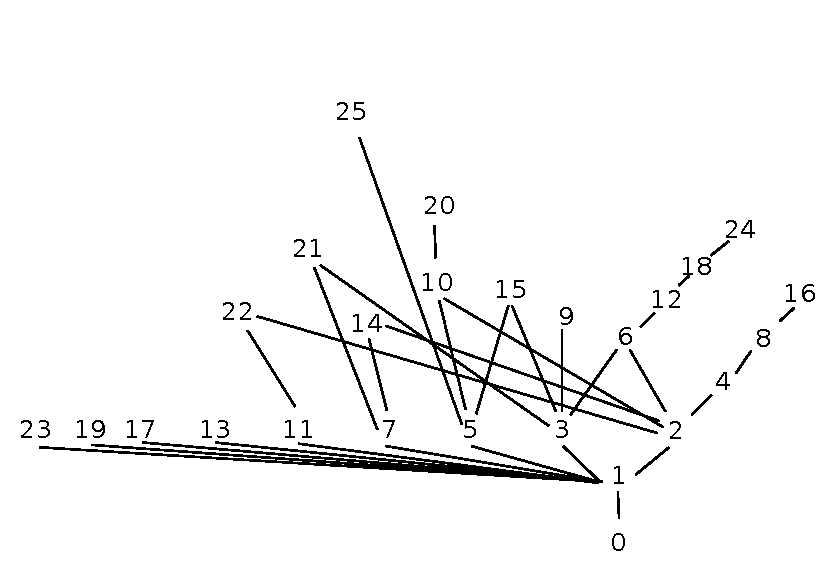
\includegraphics[width=3.0in]{5_b.pdf}}
  }
  \caption{Hasse diagram 25 elements}
\end{figure}

%6
\section{}
An equivalence relation is one that is reflexive, symmetic, and transitive.\\
If $R$ is reflexive and circular, then by definition it is reflexive.\\
If $R$ is circular, then if $aRb$, $bRc$, then $cRa$. Since it is also reflexive, $cRc$. This means that $bRc$, $cRc$, and due to the relation being circular, $cRb$. This give $bRc$ and $cRb$, which is transitivity.\\
If $R$ is circular, reflexive, and transitive, then since $aRb$ and $bRc$ gives $cRa$, and we know from transitivity that $bRc$ $cRa$ gives $bRa$, then we have symmetry with $aRb$ and $bRa$.\\

%7
\section{}
\subsection{}
$S = \{a\}$. G = $\{0\}$ (size 1)\\
$S = \{a,b\}$. G = $\{0\}, \{(a,b)\}$ (size 2)\\
$S = \{a,b,c\}$. G = $\{0\}, \{(a,b)\}, \{(a,b), (a,c)\}, \{(a,b), (a,c), (b,c)\}$ (size 4)\\
$S = \{a,b,c,d\}$. G = $\{0\}, \{(a,b)\}, \{(a,b), (a,c)\}, \{(a,b), (c,d)\}, \{(a,b), (a,c), (a,d)\},\\ \{(a,b), (a,c), (b,c)\}, \{(a,b), (b,c), (c,d)\},\\ \{(a,b), (b,c), (a,c), (c,d)\}, \{(a,b), (b,c), (c,d), (a,d), (a,c)\},\\ \{(a,b), (a,c), (a,d), (b,c), (b,d), (c,d)\}$ (size 11)\\

%8
\section{}

\[ \left( \begin{array}{cccccccc}
\ & 0 & 1 & 2 & 3 & 4 & 5 & 6\\
0 & 0 & 1 & 1 & 0 & 0 & 1 & 1\\
1 & 1 & 0 & 1 & 1 & 0 & 0 & 1\\
2 & 1 & 1 & 0 & 1 & 1 & 0 & 0\\
3 & 0 & 1 & 1 & 0 & 1 & 1 & 0\\
4 & 0 & 0 & 1 & 1 & 0 & 1 & 1\\
5 & 1 & 0 & 0 & 1 & 1 & 0 & 1\\
6 & 1 & 1 & 0 & 0 & 1 & 1 & 0\end{array} \right) \] 

\vspace{0.2in}

\[ \left( \begin{array}{cccccccc}
\ & a & b & c & d & e & f & g\\
a & 0 & 1 & 0 & 1 & 1 & 0 & 1\\
b & 1 & 0 & 1 & 0 & 1 & 1 & 0\\
c & 0 & 1 & 0 & 1 & 0 & 1 & 1\\
d & 1 & 0 & 1 & 0 & 1 & 0 & 1\\
e & 1 & 1 & 0 & 1 & 0 & 1 & 0\\
f & 0 & 1 & 1 & 0 & 1 & 0 & 1\\
g & 1 & 0 & 1 & 1 & 0 & 1 & 0\end{array} \right) \] 

%9
\section{}
\subsection{Euler Circuit}
An Euler Circuit in a graph G is a simple circuit containing every edge of G.\\
The bipartite graph $K_{m,n}$ has an Euler Circuit if $m = n$ and $m$ and $n$ are odd.\\
\subsection{Euler Path}
An Euler Circuit in a graph G is a simple path containing every edge of G.\\
The bipartite graph $K_{m,n}$ has an Euler Circuit if $m = n$ and $m$ and $n$ are even.\\
\subsection{Hamilton Circuit}
A Hamilton Circuit in a graph G is a simple circuit that passes through every vertex exactly once.\\
The bipartite graph $K_{m,n}$ has a Hamilton Circuit if $m = n$.\\
\subsection{Hamilton Path}
A Hamilton Path in a graph G is a simple path that passes through every vertex exactly once.\\
The bipartite graph $K_{m,n}$ has a Hamilton Circuit if $|m - n| \leq 1$.\\

\end{document}

%%%%%%%%%%%%%%%%%%%%%%%%%%%%%%%%%%%%%%%%%%%%%%%%%%%%%%%

%%% Local Variables: 
%%% mode: latex
%%% TeX-master: "main"
%%% End: 

